\begin{figure}[htbp]
  \centering
  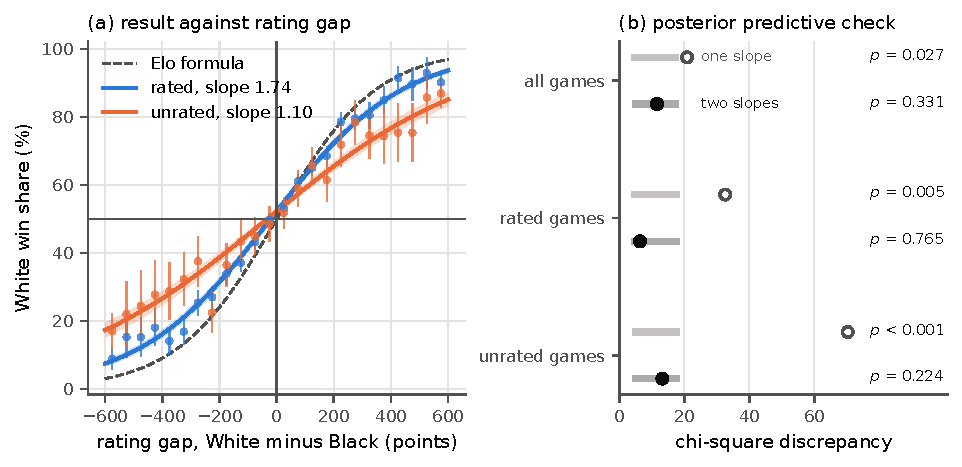
\includegraphics[width=\linewidth]{rating_slopes.pdf}
  \caption{A separate rating slope for rated and unrated games. (a): share of games won by White in bins of 50 rating points, with 90\% binomial intervals, for the 14,397 rated and 3,285 unrated decisive games; the lines and bands are the posterior mean and 90\% interval of $\operatorname{logit}^{-1}(\mu + \beta_g \Delta)$ for the average opening, and the dashed line is the expected score of the Elo formula. The rating gap predicts the result much better in rated games: the slopes differ by 0.63 (90\% interval 0.51 to 0.75). Both curves are flatter than the Elo formula: in rated games a player rated 200 points higher wins 70.4\% of decisive games (69.6 to 71.2\%), not the 76\% of the Elo formula. (b): chi-square discrepancy between wins and expected wins over the deciles of rating gap, on all games and within each group, for the model with one slope (open circles) and with two (filled); the dot is the realized discrepancy averaged over posterior draws and the bar the 90\% interval of its replicated values, with the posterior predictive $p$-value. With one slope the shape of the curve is rejected ($p = 0.027$ on all games, and lower within each group); with two slopes the misfit disappears ($p = 0.33$).}
  \label{fig:rating_slopes}
\end{figure}
